\begin{figure}[htbp]
\centering
\iffastcompile
  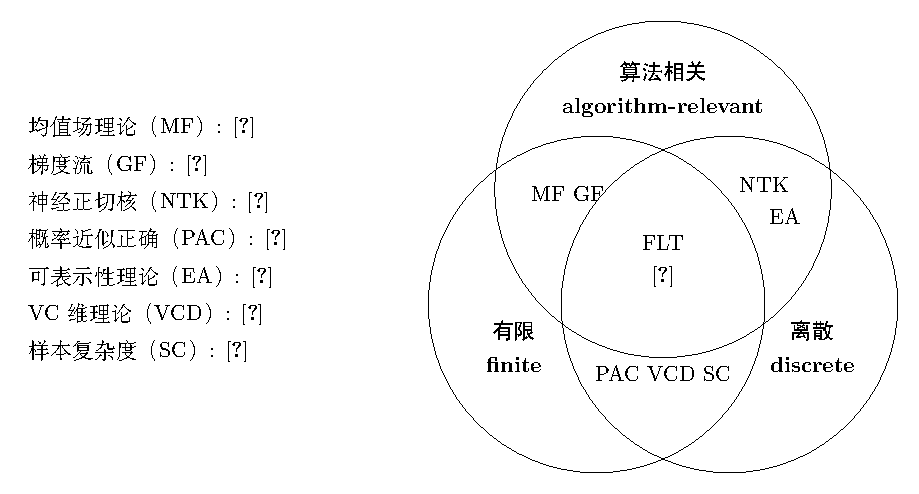
\includegraphics[width=0.99\textwidth]{figures/tikz/learning_theory_taxonomy.pdf}
\else
  \begin{tikzpicture}[scale=1.5]
  % 定义三个圆的中心
  \coordinate (A) at (0,0);
  \coordinate (B) at (1.5,0);
  \coordinate (C) at (0.75,1.3);

  % 画三个圆
  \draw[circle] (A) circle (1.9);
  \draw[circle] (B) circle (1.9);
  \draw[circle] (C) circle (1.9);

  % 标注圆的名称
  \node (finite) at ($(A)+(-0.6,-0.5)$) [above left] {\heiti{有限}};
  \node (finite_ref) at (finite.south) [below] {\textbf{finite}};
  \node (discrete) at ($(B)+(0.6,-0.5)$) [above right] {\heiti{离散}};
  \node (discrete_ref) at (discrete.south) [below] {\textbf{discrete}};
  \node (algorithm_relatedness) at ([yshift=12pt]$(C)+(0,0.7)$) [above] {\heiti{算法相关}};
  \node at (algorithm_relatedness.south) [below] {\textbf{algorithm-relevant}};

  % 圆之间的交集文字
  \node (PAC) at ($(A)!0.5!(B)+(0,-0.6)$) [below] {PAC\ VCD\ SC};
  \node (NTK) at ($(B)!0.5!(C)+(0.4,0.7)$) [right] {NTK};
  \node (EA) at ([xshift=-1pt,yshift=-10pt]NTK) [right] {EA};
  \node at ($(C)!0.5!(A)+(-0.35,0.6)$) [left] {MF\ GF};

  % 三圆交集文字
  \node (FLT) at ($(C)+(0,-0.6)$) {FLT};
  \node (FLT_ref) at (FLT.south) [below] {\cite{DBLP:conf/focs/Allen-ZhuL21}};

  % Caption
  \coordinate (caption1) at ($(A)+(-6.5,2)$);
  \node at (caption1) [right] {均值场理论（MF）: \cite{DBLP:conf/focs/Allen-ZhuL21}};
  \coordinate (caption2) at ([yshift=-12pt]caption1);
  \node at (caption2) [right] {梯度流（GF）: \cite{DBLP:conf/focs/Allen-ZhuL21}};
  \coordinate (caption3) at ([yshift=-12pt]caption2);
  \node at (caption3) [right] {神经正切核（NTK）: \cite{DBLP:conf/focs/Allen-ZhuL21}};
  \coordinate (caption4) at ([yshift=-12pt]caption3);
  \node at (caption4) [right] {概率近似正确（PAC）: \cite{DBLP:conf/focs/Allen-ZhuL21}};
  \coordinate (caption5) at ([yshift=-12pt]caption4);
  \node at (caption5) [right] {可表示性分析（EA）: \cite{DBLP:conf/focs/Allen-ZhuL21}};
  \coordinate (caption6) at ([yshift=-12pt]caption5);
  \node at (caption6) [right] {VC 维理论（VCD）: \cite{DBLP:conf/focs/Allen-ZhuL21}};
  \coordinate (caption7) at ([yshift=-12pt]caption6);
  \node at (caption7) [right] {样本复杂度（SC）: \cite{DBLP:conf/focs/Allen-ZhuL21}};
  \end{tikzpicture}
  \fi

  \caption{机器学习领域主流的理论框架示意图。左：各理论框架常见译名、英文缩写与相关参考文献。右：我们从算法相关性、有限性与离散性三个维度评价各理论框架对于不同学习任务的适用性，以突出FLT与其他理论框架的差异性。如第 \ref{sec-related-works-learning-paradigms} 小节所述，FLT 是一种算法相关、维度有限，且迭代过程离散的理论框架，适用于刻画神经网络的特征学习过程。}
  \label{fig-learning-theory-taxonomy}
\end{figure}